% article example for classicthesis.sty
\documentclass[10pt,a4paper]{article} % KOMA-Script article scrartcl
\usepackage{import}
\usepackage{xifthen}
\usepackage{pdfpages}
\usepackage{transparent}
\newcommand{\incfig}[1]{%
    \def\svgwidth{\columnwidth}
    \import{./figures/}{#1.pdf_tex}
}
\usepackage{lipsum}     %lorem ipsum text
\usepackage{titlesec}   %Section settings
\usepackage{titling}    %Title settings
\usepackage[margin=10em]{geometry}  %Adjusting margins
\usepackage{setspace}
\usepackage{listings}
\usepackage{amsmath}    %Display equations options
\usepackage{amssymb}    %More symbols
\usepackage{xcolor}     %Color settings
\usepackage{pagecolor}
\usepackage{mdframed}
\usepackage[spanish]{babel}
\usepackage[utf8]{inputenc}
\usepackage{longtable}
\usepackage{multicol}
\usepackage{graphicx}
\graphicspath{ {./Images/} }
\setlength{\columnsep}{1cm}

% ====| color de la pagina y del fondo |==== %



\begin{document}
    %========================{TITLE}====================%
    \title{{  Parcial 3 de algebra abstracta  }}
    \author{{Rodrigo Castillo (junto a Carlos y Oscar)}}
    \date{\today}

    \maketitle


    %=======================NOTES GOES HERE===================%
    \section{Sea c el código lineal de longitud $9$ cuya matriz de control es:}
    \begin{figure}[h!]
        \centering
        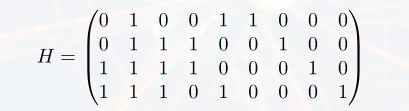
\includegraphics[width=0.8\linewidth]{matrizcontrol.png}
        \caption{matriz de control}
        \label{matriz de control}
    \end{figure}

        \subsection{a : encuentre la dimensión de $C$}
            % ====|ACA EMPIEZA EL PUNTO 1-A|====
        sabemos que si $C$ es un código lineal de longitud $n$ y dimensión $k$
        , una matrix $n-k \times  nH$ es una matriz de control para el código C
        si $wH ^{T} \iff w \in C $
        \\
        sabemos que C tiene longitud $9$
        \\
        $H$ es una matriz $4 \times 9$
        \\
        por lo tanto $n-k = 4$
        \\
        $9-k = 4$
        \\
        $k=5$
        \\
        por lo tanto $dim(C) = 5$

            % ====|ACA TERMINA EL PUNTO 1-A|==== %

        \subsection{encuentre la distancia mínima de $C$}
            % ====|ACA EMPIEZA EL PUNTO 1-b|====
        para este punto necesitamos la matris generadora de $C$ , tenemos que
        $G = (I_k A)$ y que $H = (-A ^{T} I_{n-k}$ luego ...
        \begin{equation}
            G = \begin{pmatrix}
                1 & 0 & 0 & 0 & 0 & 0 & 0 & 1 & 1
                \\
                0 & 1 & 0 & 0 & 0 & 1 & 1 & 1 & 1
                \\
                0 & 0 & 1 & 0 & 0 & 0 & 1 & 1 & 1
                \\
                0 & 0 & 0 & 1 & 0 & 0 & 1 & 1 & 0
                \\
                0 & 0 & 0 & 0 & 1 & 1 & 0 & 0 & 1
            \end{pmatrix}
        \end{equation}
        con $G$ podemos ver que la distancia mínima es $3$
            % ====|ACA TERMINA EL PUNTO 1-b|==== %

        \subsection{calcule los sindromes correspondientes a errores de
            $C$ que puede corregir}
            % ====|ACA EMPIEZA EL PUNTO 1-c|====




            % ====|ACA TERMINA EL PUNTO 1-c|==== %

        \subsection{diga si $000110011 \in C$   o no}
            % ====|ACA EMPIEZA EL PUNTO 1-d|====




            % ====|ACA TERMINA EL PUNTO 1-d|==== %

        \subsection{decodifique $110101101$}
            % ====|ACA EMPIEZA EL PUNTO 1-e|====




            % ====|ACA TERMINA EL PUNTO 1-e|==== %


























    %=======================NOTES ENDS HERE===================%

    % bib stuff
    \nocite{*}
    \addtocontents{toc}{{}}
    \addcontentsline{toc}{section}{\refname}
    \bibliographystyle{plain}
    \bibliography{../Bibliography}
\end{document}
